\documentclass{standalone}
\usepackage[T1]{fontenc}
\usepackage[latin2]{inputenc}
\usepackage[english]{babel}
\usepackage{tikz}
\usepackage{times}
\usetikzlibrary{calc,through,backgrounds,positioning,fit}
\usetikzlibrary{shapes,arrows,shadows}
 
\begin{document}
 
\centering
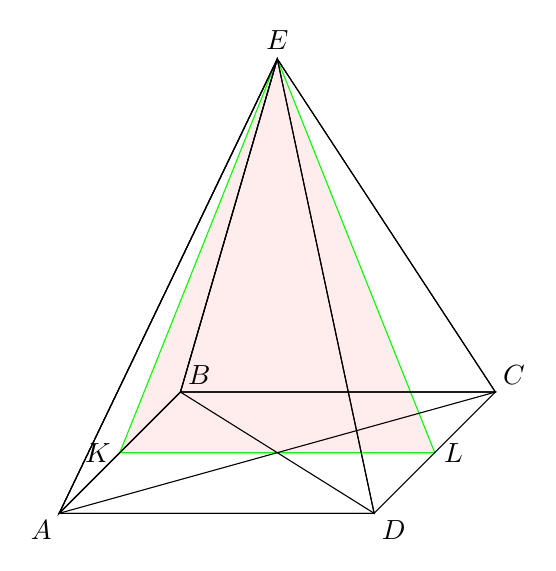
\begin{tikzpicture}[scale=1,inner sep=0.4mm]

 \coordinate (A) at (0,0,4);
 \coordinate (B) at (0,0,0);
 \coordinate (C) at (4,0,0);
 \coordinate (D) at (4,0,4);
 \coordinate (E) at (2,5,2);
 \coordinate (K) at (0,0,2);
 \coordinate (L) at (4,0,2);

\filldraw[draw=green,fill=pink!30!white] (K) -- (L)-- (E)  --cycle;
\draw[] (A) -- (B)-- (C) --(D) --cycle;
\draw[] (A) -- (B)-- (E)  --cycle;
\draw[] (A) -- (C)-- (E)  --cycle;
\draw[] (A) -- (D)-- (E)  --cycle;
\draw[] (B) -- (C)-- (E)  --cycle;
\draw[] (B) -- (D)-- (E)  --cycle;

\node at (A) [below left=2pt] {$A$};
\node at (B) [above right=2pt] {$B$};
\node at (C) [above right=2pt] {$C$};
\node at (D) [below right=2pt] {$D$};
\node at (E) [above=2pt] {$E$};
\node at (K) [left=2pt] {$K$};
\node at (L) [right=2pt] {$L$};

\end{tikzpicture}
 
\end{document}